\documentclass[a4paper]{article}
\usepackage[utf8]{inputenc}
\usepackage[english,russian]{babel}
\usepackage{indentfirst}
\usepackage{misccorr}
\usepackage{graphicx}
\graphicspath{{pics/}}
\usepackage{amsmath}
\usepackage[nottoc,numbib]{tocbibind}
\usepackage{multicol}
\usepackage{float}
\DeclareMathOperator*{\argmin}{arg\,min}
\usepackage[a4paper,margin=1.5cm]{geometry}
\usepackage{listings}
\usepackage{color}
\definecolor{dkgreen}{rgb}{0,0.6,0}
\definecolor{gray}{rgb}{0.5,0.5,0.5}
\definecolor{mauve}{rgb}{0.58,0,0.82}

\lstset{frame=tb,
  language=Java,
  aboveskip=3mm,
  belowskip=3mm,
  showstringspaces=false,
  columns=flexible,
  basicstyle={\small\ttfamily},
  numbers=none,
  numberstyle=\tiny\color{gray},
  keywordstyle=\color{blue},
  commentstyle=\color{dkgreen},
  stringstyle=\color{mauve},
  breaklines=true,
  breakatwhitespace=true,
  tabsize=3
}


\begin{document}

\begin{titlepage}
\thispagestyle{empty}

\begin{center}
\begin{figure}[htbp]
  \centering
  
\includegraphics[width=0.6\textwidth]{msu}
\end{figure}


Московский Государственный Университет им. М.В. Ломоносова

Факультет Вычислительной Математики и Кибернетики

Кафедра Автоматизации Систем Вычислительных Комплексов

\vfill
\textbf{\huge Задание по курсу "Распределённые системы"}

{\huge Отчёт}
\end{center}

\vfill
\begin{flushright}
{\large Выполнил:\\Ушаков Иван Кириллович\\421 группа\\}
\end{flushright}

\centerline{Москва, 2022 год}

\end{titlepage}
\linespread{1.7}
\setcounter{page}{2}
\large

\tableofcontents
\newpage

\section{Постановка задач}

\subsection{Задача 1: моделирование}
В транспьютерной матрице размером $4*4$, в каждом узле которой находится один процесс, необходимо выполнить операцию редукции $MPI\_MINLOC$, определить глобальный минимум и соответствующих ему индексов.
Каждый процесс предоставляет свое значение и свой номер в группе. Для всех процессов операция редукции должна возвратить значение минимума и номер первого процесса с этим значением.
Реализовать программу, моделирующую выполнение данной операции на транспьютерной матрице при помощи пересылок $MPI$ типа точка-точка.
Оценить сколько времени потребуется для выполнения операции редукции, если все процессы выдали эту операцию редукции одновременно. Время старта равно $100$, время передачи байта равно $1$ $(Ts=100,Tb=1)$. Процессорные операции, включая чтение из памяти и запись в память, считаются бесконечно быстрыми.



\subsection{Задача 2: надёжность}
Доработать MPI-программу, реализованную в рамках курса “Суперкомпьютеры и параллельная обработка данных”. Добавить контрольные точки для продолжения работы программы в случае сбоя. Реализовать один из 3-х сценариев работы после сбоя: a) продолжить работу программы только на “исправных” процессах; б) вместо процессов, вышедших из строя, создать новые MPI-процессы, которые необходимо использовать для продолжения расчетов; в) при запуске программы на счет сразу запустить некоторое дополнительное количество MPI-процессов, которые использовать в случае сбоя.\\
\textit{\textbf{В данной задаче был выбран вариант "а".}}
\newpage

\section{Пояснения к решениям}
\subsection{Моделирование}
В транспьютерной матрице размером $4*4$, в каждом узле которой находится один про-
цесс, необходимо выполнить операцию нахождения минимального значения и его координат среди $16$ чисел. Найденное минимальное значение должно быть получено
на процессе с координатами $(0,0)$.
Минимальное время оценивается через минимальное расстояние между двумя самыми дальними процессами в матрице. В нашем случае, чтобы пройти от процесса с
координатами $(0, 0)$ к процессу с координатами $(3, 3)$, необходимо сделать $6$ шагов. Это
количество шагов является минимальным, так как есть алгоритм, реализующий операцию нахождения минимума за $6$ шагов. Способ реализации:

\begin{figure}[htbp]
  \centering
  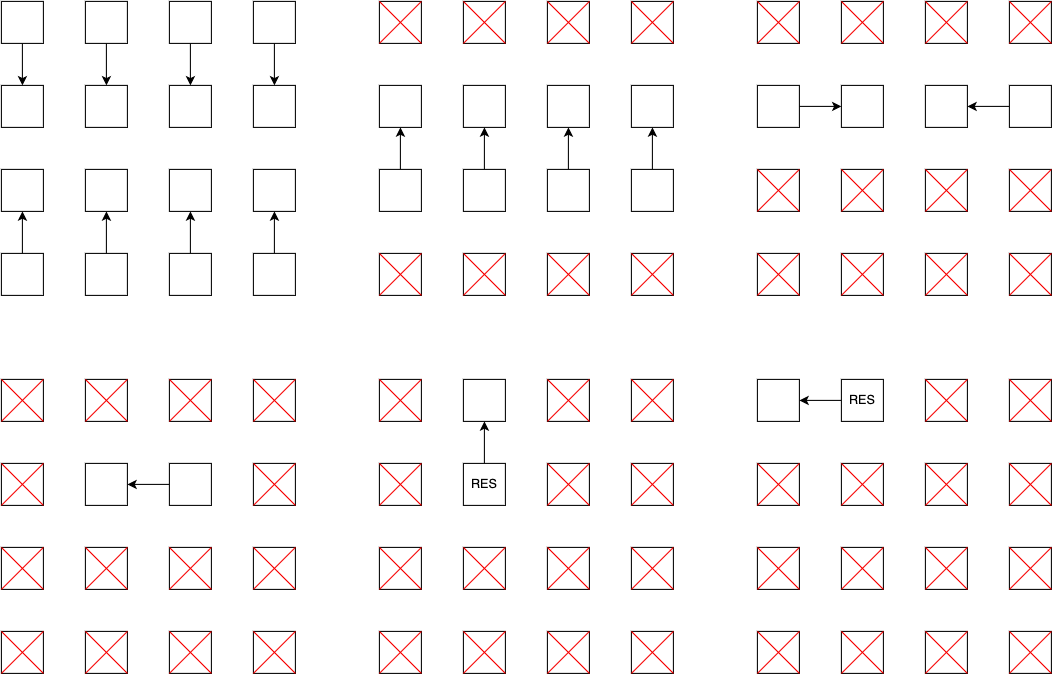
\includegraphics[width=0.6\textwidth]{graph}
\end{figure}

Данный алгоритм был реализован с помощью функций $MPI\_Send$ и $MPI\_Recv$. Получение топологии в виде транспьютерной матрицы произведено с помощью функции
$MPI\_Cart\_rank$.
Оценим время работы алгоритма. Если время старта равно $100$, время передачи байта равно $1$ $(Ts=100,Tb=1)$, то время выполнения операции рассчитывается следующим
образом:
\begin{center}
$time = num\_steps · (T s + n · T b)$
\end{center}

где n - размер передаваемого сообщения в байтах. В нашем случае сообщением является
число, размер которого может быть равен, $12$ байтам (3 числа в формате int).
Таким образом, при n = $12$, получаем:
\begin{center}
$time = 6 · (100 + 12 * 1) = 672$
\end{center}
\newpage
Пересылка сообщений была организована с помощью двух функций, которые передавали по заданному "rank"  процесса: 
\begin{lstlisting}
void send_coords_and_value(int coords[2], int value, int other_coords[2], int other_rank, MPI_Comm comm) {
    MPI_Send(coords, 2, MPI_INT, other_rank, 0, comm);
    MPI_Send(&value, 1, MPI_INT, other_rank, 0, comm);
}
void receive_coords_and_value(int coords[2], int *value, int *other_coords, int other_rank, MPI_Comm comm){
    MPI_Recv(other_coords, 2, MPI_INT, other_rank, 0, comm, MPI_STATUS_IGNORE);
    MPI_Recv(value, 1, MPI_INT, other_rank, 0, comm, MPI_STATUS_IGNORE);
}
\end{lstlisting}

Создание транспьютерной матрицы с помощью \textit{MPI\_Cart\_create}:
\begin{lstlisting}
 MPI_Cart_create(MPI_COMM_WORLD, 2, size, periodic, 0, &comm);
\end{lstlisting}

На первом шаге алгоритма мы пересылаем сообщения из первого ряда во второй и из четвёртого в третий. Поэтому в 0 и 3 координате по вертикали мы вызываем функцию \textit{send\_coords\_and\_value}, а в 1 и 2 координате по вертикале мы вызываем функцию \textit{receive\_coords\_and\_value}. Таким образом процессы в 0 и 3 строке отправляют текущий минимум в строки 1 и 2, а те их получают и заменяют минимум и координаты минимума в случае необходимости. Функция \textit{MPI\_Cart\_rank} позволяет получить rank процесса по его координатам. Аналогично в остальных шагах.

Первый шаг:
\begin{lstlisting}
 other_coords[1] = coords[1];
    
    switch(coords[0]) {
        case 0:
            other_coords[0] = coords[0] + 1;
            MPI_Cart_rank(comm, other_coords, &other_rank);
            send_coords_and_value(result_coords, a, other_coords, other_rank, comm);
        break;
        case 3:
            other_coords[0] = coords[0] - 1;
            MPI_Cart_rank(comm, other_coords, &other_rank);
            send_coords_and_value(result_coords, a, other_coords, other_rank, comm);
        break;
            
        case 1:
            other_coords[0] = coords[0] - 1;
            MPI_Cart_rank(comm, other_coords, &other_rank);
            receive_coords_and_value(coords, &result, other_coords, other_rank, comm);
            goto Better_res;
        break;
        case 2:
            other_coords[0] = coords[0] + 1;
            MPI_Cart_rank(comm, other_coords, &other_rank);
            receive_coords_and_value(coords, &result, other_coords, other_rank, comm);
        Better_res:
            if (result < a) {
                a = result;
                result_coords[0] = other_coords[0];
                result_coords[1] = other_coords[1];
            }
        break;
        default:
        break;
    }
    MPI_Barrier(comm);
\end{lstlisting}

\newpage
Второй шаг алгоритма:
\begin{lstlisting}
switch(coords[0]) {
        case 1:
            other_coords[0] = coords[0] + 1;
            MPI_Cart_rank(comm, other_coords, &other_rank);
            receive_coords_and_value(coords, &result, other_coords, other_rank, comm);
            
            if (result < a) {
                a = result;
                result_coords[0] = other_coords[0];
                result_coords[1] = other_coords[1];
            }
        break;
        case 2:
            other_coords[0] = coords[0] - 1;
            MPI_Cart_rank(comm, other_coords, &other_rank);
            send_coords_and_value(result_coords, a, other_coords, other_rank, comm);
        break;
        default:
        break;
    }
    MPI_Barrier(comm);
\end{lstlisting}

\newpage
Третий шаг алгоритма:
\begin{lstlisting}
if (coords[0] == 1 && (coords[1] == 0 || coords[1] == 3)) {
        other_coords[0] = coords[0];
        if (coords[1] == 0) {
            other_coords[1] = coords[1] + 1;
        } else {
            other_coords[1] = coords[1] - 1;
        }
        MPI_Cart_rank(comm, other_coords, &other_rank);
        send_coords_and_value(result_coords, a, other_coords, other_rank, comm);
    }
    
    if (coords[0] == 1 && (coords[1] == 1 || coords[1] == 2)) {
        other_coords[0] = coords[0];
        if (coords[1] == 1) {
            other_coords[1] = coords[1] - 1;
        } else {
            other_coords[1] = coords[1] + 1;
        }
        MPI_Cart_rank(comm, other_coords, &other_rank);
        receive_coords_and_value(coords, &result, other_coords, other_rank, comm);
        
        if (result < a) {
            a = result;
            result_coords[0] = other_coords[0];
            result_coords[1] = other_coords[1];
        }
    }
    MPI_Barrier(comm);
\end{lstlisting}

\newpage
Четвёртый шаг алгоритма:
\begin{lstlisting}
if (coords[0] == 1 && coords[1] == 3) {
        other_coords[0] = coords[0];
        other_coords[1] = 1;
        MPI_Cart_rank(comm, other_coords, &other_rank);
        send_coords_and_value(result_coords, a, other_coords, other_rank, comm);
    }
    if (coords[0] == 1 && coords[1] == 1) {
        other_coords[0] = coords[0];
        other_coords[1] = 3;
        MPI_Cart_rank(comm, other_coords, &other_rank);
        receive_coords_and_value(coords, &result, other_coords, other_rank, comm);
        if (result < a) {
            a = result;
            result_coords[0] = other_coords[0];
            result_coords[1] = other_coords[1];
        }
    }
    MPI_Barrier(comm);
\end{lstlisting}

Пятый шаг алгоритма
\begin{lstlisting}
if (coords[0] == 1 && coords[1] == 1) {
        other_coords[0] = 0;
        other_coords[1] = 1;
        MPI_Cart_rank(comm, other_coords, &other_rank);
        send_coords_and_value(result_coords, a, other_coords, other_rank, comm);
    }
    if (coords[0] == 0 && coords[1] == 1) {
        other_coords[0] = 1;
        other_coords[1] = 1;
        MPI_Cart_rank(comm, other_coords, &other_rank);
        receive_coords_and_value(coords, &result, other_coords, other_rank, comm);
        if (result < a) {
            a = result;
            result_coords[0] = other_coords[0];
            result_coords[1] = other_coords[1];
        }
    }
    MPI_Barrier(comm);
\end{lstlisting}

\newpage
Шестой шаг алгоритма:
\begin{lstlisting}
if (coords[0] == 0 && coords[1] == 1) {
        other_coords[0] = 0;
        other_coords[1] = 0;
        MPI_Cart_rank(comm, other_coords, &other_rank);
        send_coords_and_value(result_coords, a, other_coords, other_rank, comm);
    }
    if (coords[0] == 0 && coords[1] == 0) {
        other_coords[0] = 0;
        other_coords[1] = 1;
        MPI_Cart_rank(comm, other_coords, &other_rank);
        receive_coords_and_value(coords, &result, other_coords, other_rank, comm);
        if (result < a) {
            a = result;
            result_coords[0] = other_coords[0];
            result_coords[1] = other_coords[1];
        }
    }
    
    MPI_Barrier(comm);
\end{lstlisting}


\newpage
\subsection{Надёжность}
Программа, написанная в рамках курса СКиПОД решала задачу вычисления интеграла методом Монте-Карло. 
При запуске должен быть задан параметр --- количество итераций для рассчёта интеграла. Саму формулу можно изменить в исходниках программы:

\begin{lstlisting}
long double cur_function(long double x)
{
    return x*x + x*x*x;
}

\end{lstlisting}


 Для начала нам необходимо написать функцию, которая будет срабатывать в случае возникновения сбоя. В варианте \textit{а)} задания после сбоя используются только исправные процессы. В  функции-обработчике и происходит нахождение отказавшей задачи и повторный запуск уже с оставшимся количеством процессов:

\begin{lstlisting}
static void errhandler(MPI_Comm* pcomm, int* perr, ...) {
    error_occured = 1;
    int err = *perr;
    char errstr[MPI_MAX_ERROR_STRING];
    int size, nf, len;
    MPI_Group group_f;
    /*
     Here we get nuymber of crashed processes, error type and change constant, to make formula correct without crashed processor
     */
    MPI_Comm_size(main_comm, &size);
    MPIX_Comm_failure_ack(main_comm);
    MPIX_Comm_failure_get_acked(main_comm, &group_f);
    MPI_Group_size(group_f, &nf);
    MPI_Error_string(err, errstr, &len);
    N -= nf*(N/numprocs);
    /*
     Create new communicator without crashed processor
     */
    MPIX_Comm_shrink(main_comm, &main_comm);
    MPI_Comm_rank(main_comm, &rank);
    MPI_Comm_size(main_comm,&numprocs);

\end{lstlisting}


\newpage
Затем в функции main обозначить функцию как обработчик в случае ошибок:
\begin{lstlisting}
 	/*
     Set error handler
     */
    MPI_Errhandler errh;
    MPI_Comm_create_errhandler(errhandler, &errh);
    MPI_Comm_set_errhandler(main_comm, errh);
\end{lstlisting}

Необходимо также добавить контрольную точку, чтобы после расчётов, если выяснится, что произошёл сбой, то результат не может быть верным, из-за чего необходимо пересчитать данные на уже только исправных процессах:\\ 
\begin{lstlisting}
	/*
	    Summing everything in varaible drobSum and goto checkpoint 
	    if there was an error (because varaible numproc has changed)
    */
 checkpoint:
    MPI_Barrier(main_comm);
    for (long long int j = 0; j < N/numprocs; j++){
        drobSum += cur_function(rand_point(leftBorder, rightBorder));
        if (error_occured == 1) {
            error_occured = 0;
            goto checkpoint;
        }
    }
    if (error_occured == 1) {
        error_occured = 0;
        goto checkpoint;
    }

\end{lstlisting}

Ну и последнее -- это искусственно смоделировать отказ c помощью \textit{SIGKILL}:\\ 
\begin{lstlisting}
	/*
    Modelling fault
    */
    MPI_Barrier(main_comm);
    if (myid == KILLED_PROCESS) {
            raise(SIGKILL);
    }
    MPI_Barrier(main_comm);

\end{lstlisting}


В остальном интеграл продолжает считаться так же как и в задании из курса СКиПОД


\section{Исходный код}
В рамках задания по курсу "Распределённые системы" были реализованы две параллельные программы, исходный код которых можно найти в репозитории \\
\textit{https://github.com/Ushuaya/Skipod\_2\_or\_Distributed\_systemns.git}. 
\\Кроме того, файлы с исходными текстами программ прикреплены в трекере на сайте \textit{dvmh.keldysh.ru}.


\end{document}

